\documentclass[a4paper, 10pt]{article}
\usepackage[utf8]{inputenc} % Change according your file encoding
\usepackage{graphicx}
\usepackage{url}
\usepackage{amsmath}
\usepackage{mathtools}
\usepackage{mathrsfs}
\usepackage{amsfonts}
\usepackage{bbm}
\usepackage{amsthm}
\usepackage{amssymb}
\usepackage{fancyhdr}
\usepackage{setspace}
\usepackage{tabularx}
\usepackage{tikz}
\usetikzlibrary{arrows,positioning}
\usepackage[a4paper, left=2cm, right=2cm, top=2.5cm, bottom=2cm]{geometry}

\pagestyle{fancy}
\fancyhf{}
\rhead{Tuesday, December 19th}
\lhead{Víctor Mart\'in, Pablo Oviedo, and Carlos Segarra - DAG: Sheet 2}
\cfoot{\thepage}

\newtheorem{obs}{Observation}
\newtheorem{theorem}{Theorem}
\newtheorem*{theoremstar}{Theorem}

\theoremstyle{definition} % amsthm only
\newtheorem{definition}{Definition}

%\newtheorem{def}{Definition}

\newcommand{\espai}{\vspace{3mm}}
\newcommand{\cT}{\mathcal{T}}
\newcommand{\cA}{\mathcal{A}}
\newcommand{\I}{\mathscr{I}}
\newcommand{\B}{\mathscr{B}}
\newcommand{\C}{\mathscr{C}}
\newcommand{\F}{\mathscr{F}}
\newcommand{\RR}{\mathbbm{R}}
\newcommand{\aaa}{\mathbf{a}}

% Listings for Problem 5
\usepackage{listings,lstautogobble}
\definecolor{background}{rgb}{0.95,0.95,0.92}
\lstset{
    basicstyle=\footnotesize\ttfamily,
    xleftmargin=1pt,
    showstringspaces=false,
    breaklines=true,
    frame = tblr,
    autogobble = true,
    backgroundcolor=\color{background},
    commentstyle=\color{gray},
}
\lstdefinestyle{python}{
    language = Python,
    numbers = left,
    numbersep=5pt,
    keywordstyle=\color{purple},
    morekeywords={rand,timer,define},
    numberstyle=\tiny\color{gray!80},
    emphstyle=\color{red!50!blue},
    emph={addConstr, Model, addVars, GRB, gp}
}

\begin{document}
\onehalfspacing
\tikzstyle{vertice}=[circle, draw, fill=black!50, inner sep = 0pt, minimum width=4pt]

\textbf{\Large Discrete and Algorithmic Geometry: Sheet 2}

\vspace{20pt}

\textbf{\textit{(6) The permutohedron $\Pi^{n-1}$ is the convex hull of all $n!$ permutations of the vector $(1,2,\dots,n)$. For $n\ge3$, show that $\dim\Pi^{n-1}=n-1$, that $f_{n-2}(\Pi^{n-1}) = 2^n-2$, and $f_1(\Pi^{n-1}) = \tfrac12 (n-1)n!$. If you like, show that $f_k(\Pi^{n-1}) = k!\{{n\atop k}\} = \sum_{i=0}^k(-1)^i\binom{k}{i}(k-i)^n$.}}

\vspace{5pt}

WRITE HERE


\vspace{5pt}

\begin{center}
    \rule{5cm}{0.4pt}
\end{center}

\newpage

\textbf{\textit{(5) Let $\cT=\{\sigma_1,\dots,\sigma_m\}$ be a triangulation of a full-dimensional point configuration $\cA=(\aaa_1,\dots,\aaa_n)\subset\RR^d$ of $n$~points, where we consider the $\sigma_i\in\binom{[n]}{d+1}$ to be index sets. Let $R^{\text{int}}$ be the set of interior ridges, defined to be intersections $\rho = \rho_{ij} = \sigma_i\cap\sigma_j$ of two facets of~$\cT$ such that the affine span of the points of~$\cA$ indexed by~$\rho$ has dimension~$d-1$. (In the triangulations of~Figure~\ref{fig:triangs1}, they are the interior edges.)}}

  \begin{figure}[htbp]
    \centering
    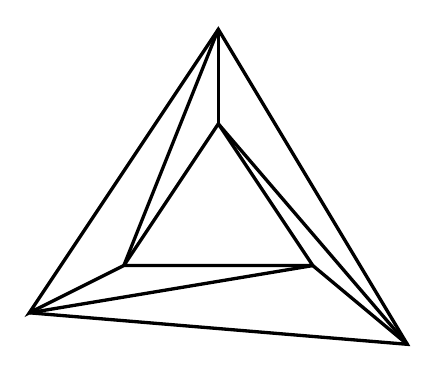
\begin{tikzpicture}[scale=.4]
      \coordinate (1) at (0,0);
      \coordinate (2) at (12,-1);
      \coordinate (3) at (6,9);
      \coordinate (4) at (3,1.5);
      \coordinate (5) at (9,1.5);
      \coordinate (6) at (6,6);

      \draw[very thick] (1)--(2)--(3)--(1)--(4)--(5)--(6)--(4);
      \draw[very thick] (2)--(5);
      \draw[very thick] (3)--(6);

      \draw[very thick] (1)--(5);
      \draw[very thick] (2)--(6);
      \draw[very thick] (3)--(4);
    \end{tikzpicture}
    \qquad
    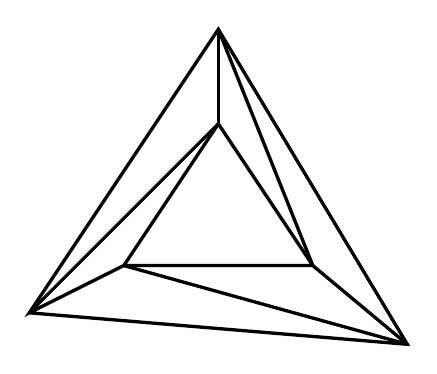
\begin{tikzpicture}[scale=.4]
      \coordinate (1) at (0,0);
      \coordinate (2) at (12,-1);
      \coordinate (3) at (6,9);
      \coordinate (4) at (3,1.5);
      \coordinate (5) at (9,1.5);
      \coordinate (6) at (6,6);

      \draw[very thick] (1)--(2)--(3)--(1)--(4)--(5)--(6)--(4);
      \draw[very thick] (2)--(5);
      \draw[very thick] (3)--(6);

      \draw[very thick] (2)--(4);
      \draw[very thick] (3)--(5);
      \draw[very thick] (1)--(6);
    \end{tikzpicture}    
    \caption{Two triangulations.
    View the source code for the coordinates of the points.}
    \label{fig:triangs1}
  \end{figure}

\begin{enumerate}
  \item
    For a vector $\omega\in\RR^n$, lift the points in $\cA$ to heights~$\omega$, so that
    $\cA^\omega=\big(\binom{\aaa_1}{\omega_1},\dots,\binom{\aaa_n}{\omega_n}\big)$.
    For each interior ridge $\rho=\sigma_i\cap\sigma_j\in R^{\text{int}}$,
    formulate the folding condition that expresses that $\rho$ indexes a face of the lower convex hull of~$\cA^\omega$,
    in terms of the coordinates of the~$\aaa_i$ and~$\omega$.
    Your folding condition should be an inequality that is linear in each height~$\omega_i$.

To formulate the folding condition, we make use of Definition 7.4 in Rheka R. Thomas~\footnote{Rekha R. Thomas. Lectures in geometric combinatorics., volume 33 of Student Mathematical Library. Providence, RI: American Mathematical Society (AMS); Princeton, NJ: Institute for Advanced Studies, 2006.}:
        \begin{equation*}
            bla
        \end{equation*}

  \item
    Write code that takes the coordinates of the $\aaa_i$ and the facets $\sigma_i$ of a triangulation as input,
    and outputs the set of folding conditions in a text file in
    LP file format.

  \item
    Download a linear programming software such as
    \texttt{gurobi},
    \texttt{cplex} or
    \texttt{scip}/\texttt{soplex}
    and check explicitly whether there exists a choice of heights $\omega$ that induces each of the triangulations of Figure~\ref{fig:triangs1}.

  \item
    Using this code,
    check that the triangulation of the $4$-dimensional cube from~\cite{deLoera96}
    given by the files \texttt{4-cube.vertices} and \texttt{4-cube.triangulation}
    is non-regular, i.e., it does not come from a lifting to~$\RR^5$.
    If you like, download and play with TOPCOM.
  \end{enumerate}


\vspace{5pt}

\begin{center}
    \rule{5cm}{0.4pt}
\end{center}

\newpage

\textbf{\textit{(6) The permutohedron $\Pi^{n-1}$ is the convex hull of all $n!$ permutations of the vector $(1,2,\dots,n)$. For $n\ge3$, show that $\dim\Pi^{n-1}=n-1$, that $f_{n-2}(\Pi^{n-1}) = 2^n-2$, and $f_1(\Pi^{n-1}) = \tfrac12 (n-1)n!$. If you like, show that $f_k(\Pi^{n-1}) = k!\{{n\atop k}\} = \sum_{i=0}^k(-1)^i\binom{k}{i}(k-i)^n$.}}

\vspace{5pt}

WRITE HERE


\vspace{5pt}

\begin{center}
    \rule{5cm}{0.4pt}
\end{center}

\end{document}
